\documentclass[border=1pt]{standalone}

\usepackage{tikz}

\usetikzlibrary{calc}

\usepackage{amsmath}
\usepackage{luatexja}

\begin{document}

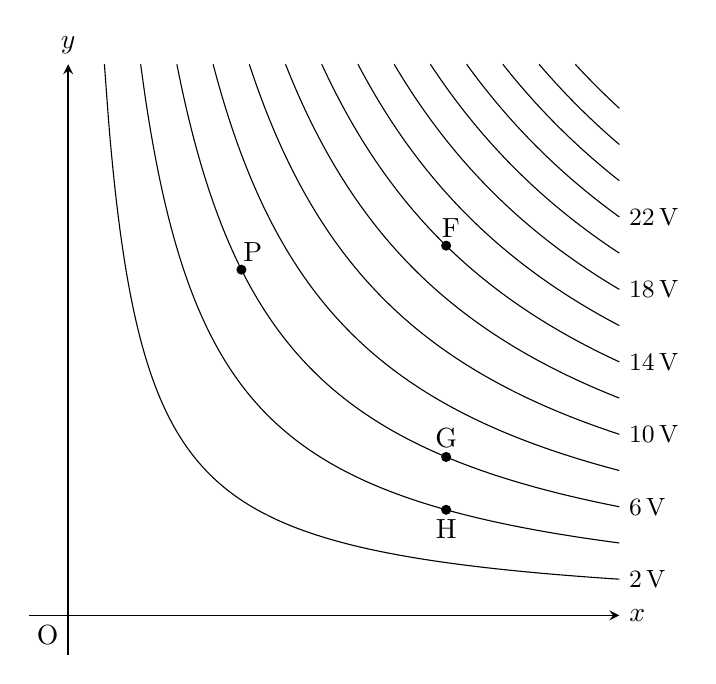
\begin{tikzpicture}[>=stealth]

    % --- 1. 変数定義 ---
    \pgfmathsetmacro{\xmax}{7}
    \pgfmathsetmacro{\ymax}{7}
    \pgfmathsetmacro{\a}{3.22}
    
    \pgfmathsetmacro{\xa}{2.2}
    \pgfmathsetmacro{\xb}{4.8}
    \pgfmathsetmacro{\h}{\a*2/\xb}
    \pgfmathsetmacro{\g}{\a*3/\xb}
    \pgfmathsetmacro{\f}{\a*7/\xb}
    \pgfmathsetmacro{\p}{\a*3/\xa} 

    % --- 2. 座標軸 ---
    \draw[->, semithick] (-.5,0) -- (\xmax,0) node[right] {$x$};
    \draw[->, semithick] (0,-.5) -- (0,\ymax) node[above] {$y$};
    \node at (0,0) [below left] {O};

    % --- 3. 等電位線（反比例群）の描画 ---
    \foreach \k in {1,2,...,14} {
        % yが巨大になりすぎないよう、左端の開始x座標を制限
        \pgfmathsetmacro{\kx}{max(0.35, \a*\k/\ymax)}
        \draw[thin, domain=\kx:\xmax, samples=100, smooth] 
            plot(\x, {\a*\k/\x});
    }

    % --- 4. 電位ラベルの追加 (グラフの右端に整列) ---
    \foreach \v/\val in {1/2, 3/6, 5/10, 7/14, 9/18, 11/22} {
        \node at (\xmax, \a*\v/\xmax) [right] {\small{\val\,V}};
    }

    % --- 5. 指定点（観測点）のプロット ---
    \filldraw[fill=black] (\xb,\h) circle (1.6pt) node[below] {H};
    \filldraw[fill=black] (\xb,\g) circle (1.6pt) node[above] {G};
    \filldraw[fill=black] (\xb,\f) circle (1.6pt) node[above=2.3mm,right=-1.8mm] {F};
    \filldraw[fill=black] (\xa,\p) circle (1.6pt) node[above=2.3mm,right=-1mm] {P};

\end{tikzpicture}

\end{document}
